
\subsection{Experiment Settings}
\begin{itemize}
    \item cpu:
    \item ram:
    \item ssd:
    \item rocksdb:
\end{itemize}




\begin{figure}
    % \centering
    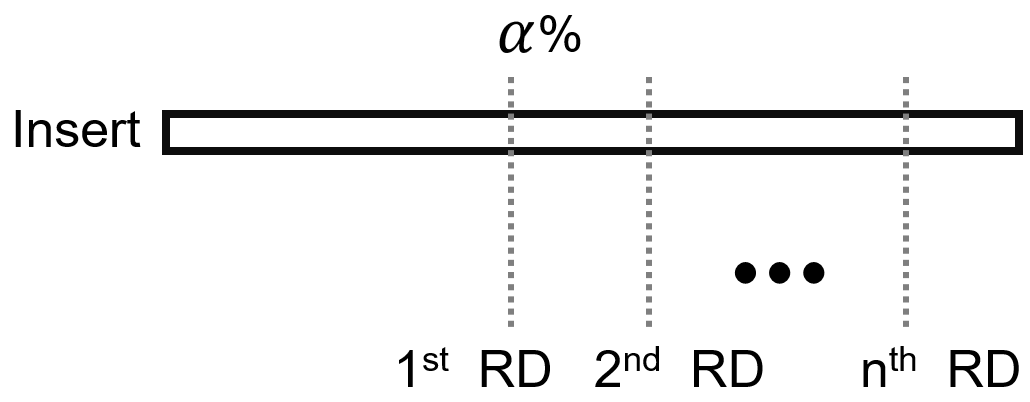
\includegraphics[width=0.2 \textwidth]{Figures/workload.png}
    \Description[<short description>]{<long description>}
    \caption{\label{fig:workload} The first RD is inserted at the $ \alpha  $ of the total insert, and all the following RDs are equally separated between the first RD the end of the insert workload.}
\end{figure}
    

workload settings: \\
    Workload composed 2 parts, the first part is the insert workload, the second part is the query workload. Within the insertion workload, there're entry insert andRD while the RDs are equally dirstributed with an variable $ \alpha $ that decides where the first RD starts at, which is shown in Figure .

    In \ref{fig:workload}.




% \begin{figure}[h!]
% % \centering
% 
\includegraphics[width=0.25 \textwidth]{Figures/T2_P32_B4_E1024_128p0MB_alpha0p1_elapse_time_on_currently_deleted_keys.png}
% % 
\includegraphics[scale=0.1]{Figures/T2_P32_B4_E1024_128p0MB_alpha0p1_elapse_time_on_currently_deleted_keys.png}
% \Description[<short description>]{<long description>}
% \caption{\label{fig:elapsed_time__currently_deleted_keys__Skyline} Elapsed time of testing on all of the deleted keys when $\alpha$ = 0.9, T = 2, P =32, E = 1024. From left to right separated into 3 groups [(g1,g2,g3), (g4,g5,g6), (g7,g8,g9)], each of them has selectivity 0.001, 0.01, 0.1 respectively.  While (g1,g4,g7) has 10\% of total keys deleted and the middle three (g2,g5,g8) have 50\%, whereas the tallest ones (g3,g6,g9) have 90\% keys deleted.}
% \end{figure}




\begin{figure}
% \centering
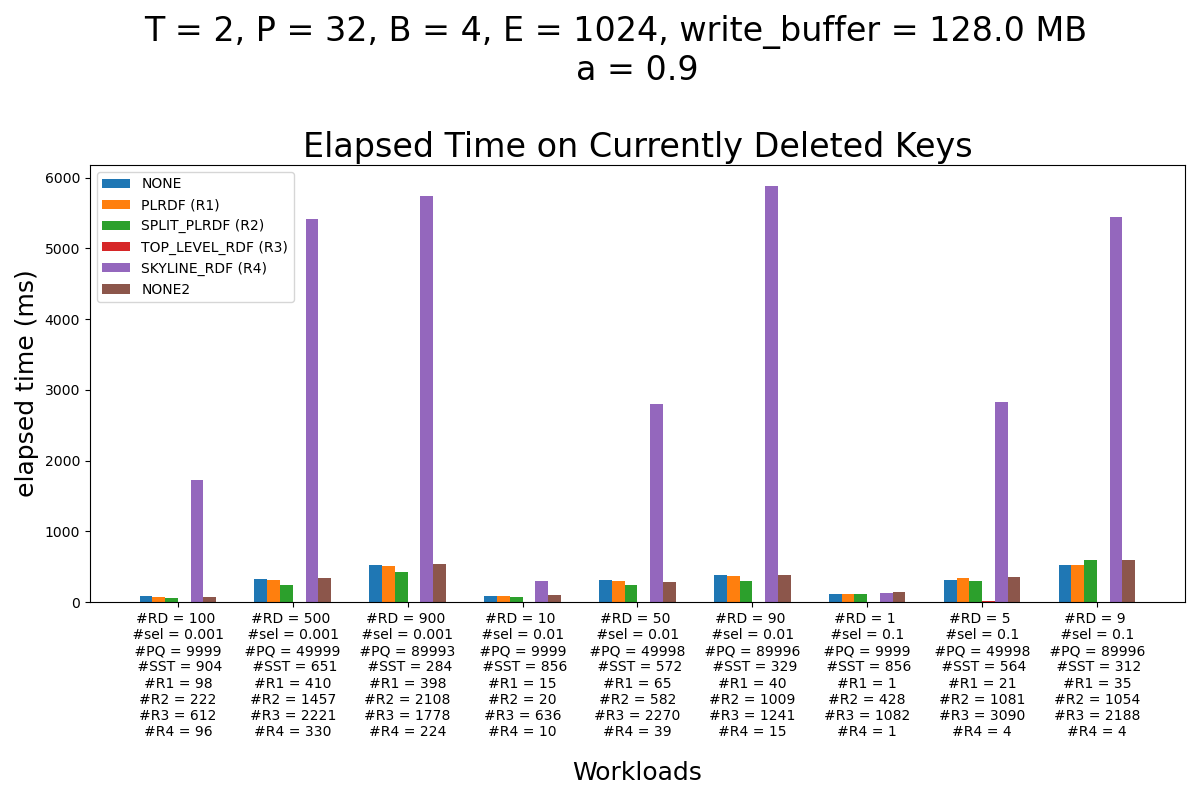
\includegraphics[width=0.45 \textwidth]{Figures/T2_P32_B4_E1024_128p0MB_alpha0p9/T2_P32_B4_E1024_128p0MB_alpha0p9_elapse_time_on_currently_deleted_keys__Skyline.png}
\Description[<short description>]{<long description>}
\caption{ Elapsed time of testing on all of the deleted keys when $\alpha$ = 0.9, T = 2, P =32, E = 1024. From left to right separated into 3 groups [(g1,g2,g3), (g4,g5,g6), (g7,g8,g9)], each of them has selectivity 0.001, 0.01, 0.1 respectively.  While (g1,g4,g7) has 10\% of total keys deleted and the middle three (g2,g5,g8) have 50\%, whereas the tallest ones (g3,g6,g9) have 90\% keys deleted.}
\label{fig:elapsed_time__currently_deleted_keys__Skyline}
\end{figure}



\begin{figure}
% \centering
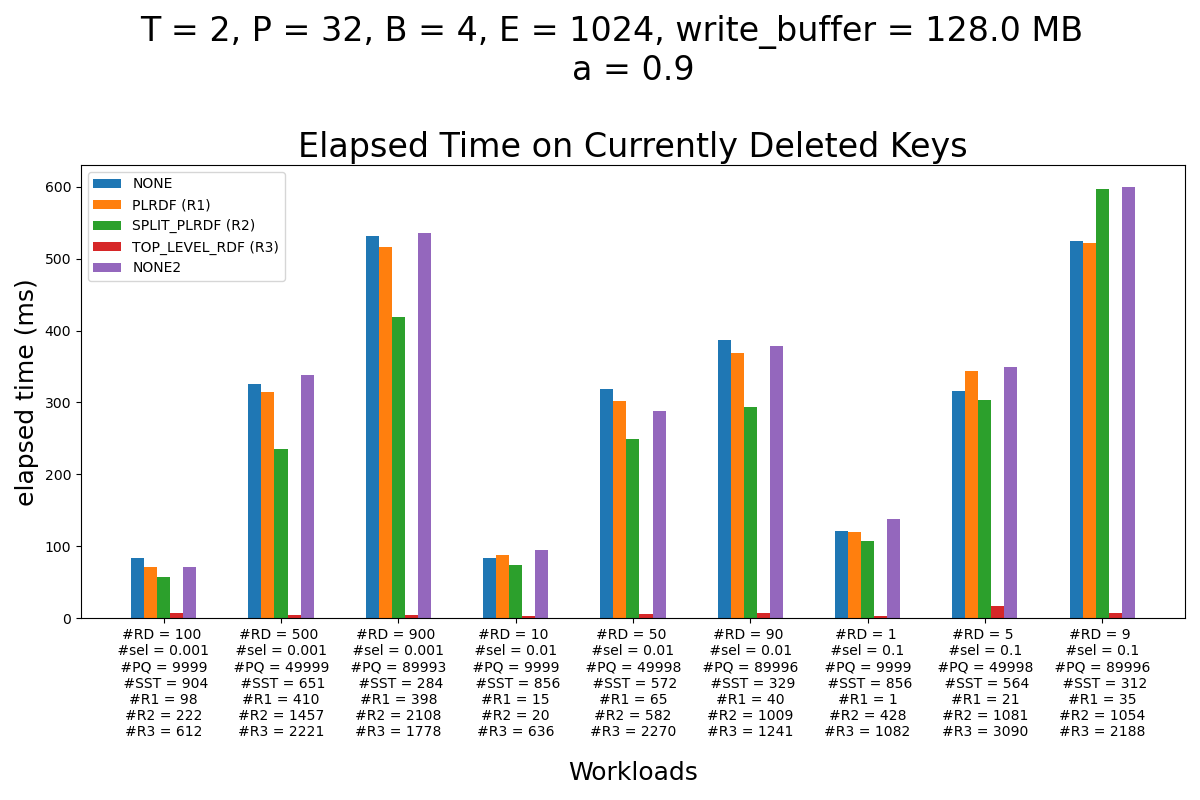
\includegraphics[width=0.45 \textwidth]{Figures/T2_P32_B4_E1024_128p0MB_alpha0p9/T2_P32_B4_E1024_128p0MB_alpha0p9_elapse_time_on_currently_deleted_keys.png}
\Description[<short description>]{<long description>}
\caption{Elapsed time of testing on all of the deleted keys without Skyline when $\alpha$ = 0.9, T = 2, P =32, E = 1024. From left to right separated into 3 groups [(g1,g2,g3), (g4,g5,g6), (g7,g8,g9)], each of them has selectivity 0.001, 0.01, 0.1 respectively.  While (g1,g4,g7) has 10\% of total keys deleted and the middle three (g2,g5,g8) have 50\%, whereas the tallest ones (g3,g6,g9) have 90\% keys deleted.}
\label{fig:elapsed_time__currently_deleted_keys} 
\end{figure}


\begin{figure}
    % \centering
    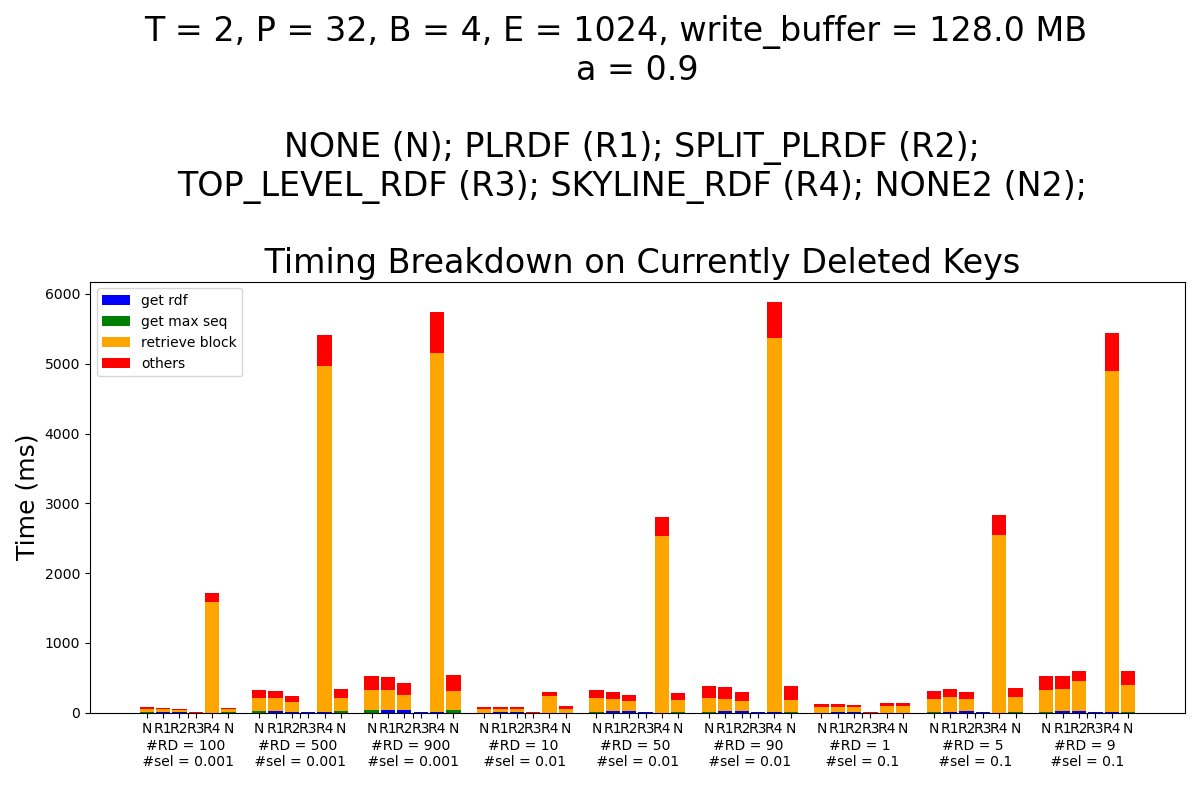
\includegraphics[scale=0.25]{Figures/T2_P32_B4_E1024_128p0MB_alpha0p9/T2_P32_B4_E1024_128p0MB_alpha0p9_timing_breakdown_on_currently_deleted_keys__Skyline.png}
    \Description[<short description>]{<long description>}
    \caption{ Timing breakdown of testing on all of the deleted keys when $\alpha$ = 0.9, T = 2, P =32, E = 1024. Over 9 workloads.}
    \label{fig:timing_breakdown__currently_deleted_keys__Skyline}
\end{figure}


\begin{figure}
    % \centering
    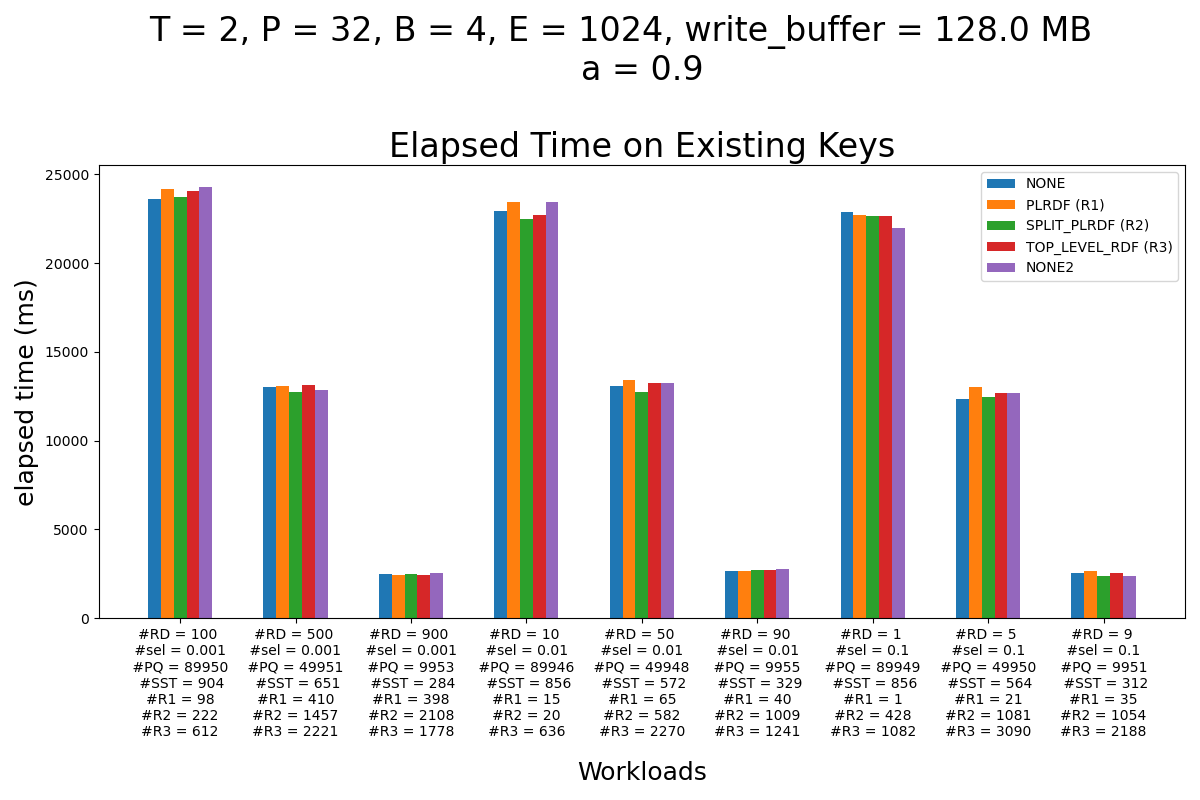
\includegraphics[scale=0.25]{Figures/T2_P32_B4_E1024_128p0MB_alpha0p9/T2_P32_B4_E1024_128p0MB_alpha0p9_elapse_time_on_existing_keys.png}
    \Description[<short description>]{<long description>}
    \caption{Elapsed time of testing on all of the existing keys when $\alpha$ = 0.9, T = 2, P =32, E = 1024. Over 9 workloads.}
    \label{fig:elapsed_time__existing_keys__Skyline} 
\end{figure}


\begin{figure}
    % \centering
    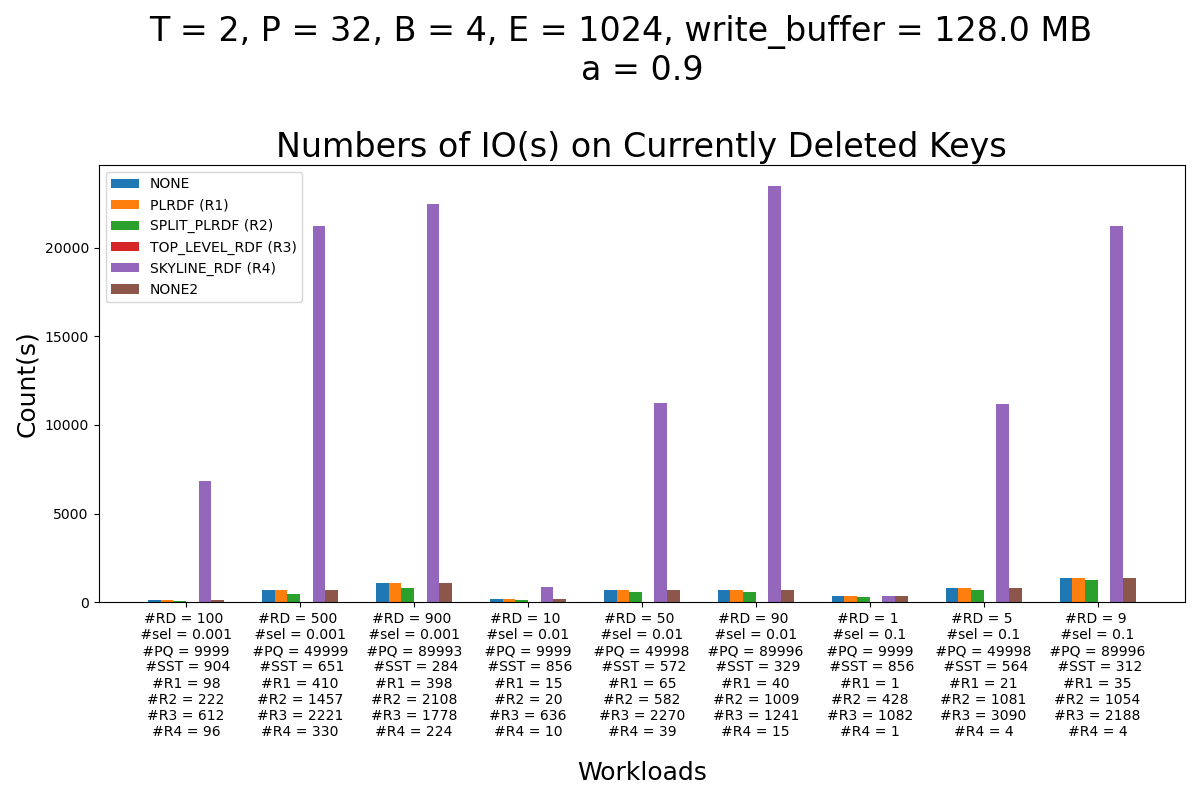
\includegraphics[scale=0.25]{Figures/T2_P32_B4_E1024_128p0MB_alpha0p9/T2_P32_B4_E1024_128p0MB_alpha0p9_IOs_on_currently_deleted_keys__Skyline.png}
    \Description[<short description>]{<long description>}
    \caption{ Elapsed time of testing on all of the existing keys when $\alpha$ = 0.9, T = 2, P =32, E = 1024. Over 9 workloads.}
    \label{fig:IO__currently_deleted_keys__Skyline}
\end{figure}


\begin{figure}
    % \centering
    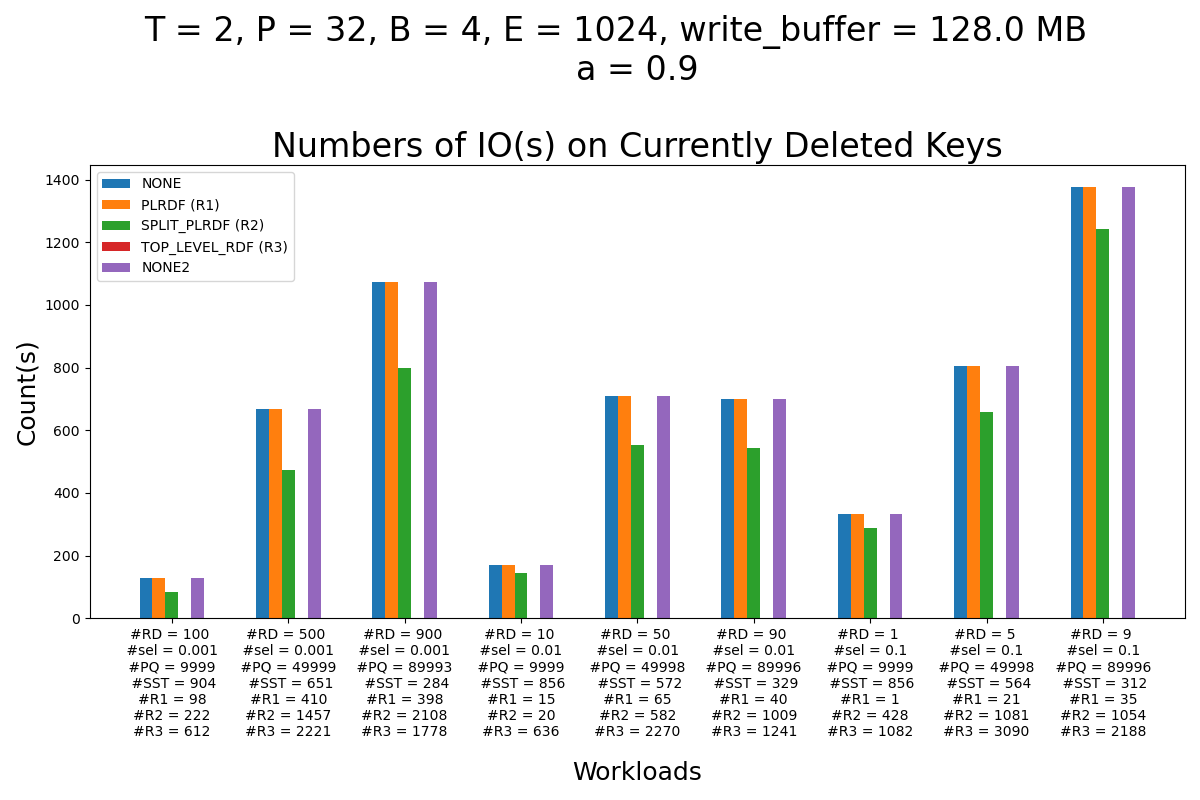
\includegraphics[scale=0.25]{Figures/T2_P32_B4_E1024_128p0MB_alpha0p9/T2_P32_B4_E1024_128p0MB_alpha0p9_IOs_on_currently_deleted_keys.png}
    \Description[<short description>]{<long description>}
    \caption{ Elapsed time of testing on all of the existing keys when $\alpha$ = 0.9, T = 2, P =32, E = 1024. Over 9 workloads.}
    \label{fig:IO__currently_deleted_keys}
\end{figure}


\begin{figure}
    % \centering
    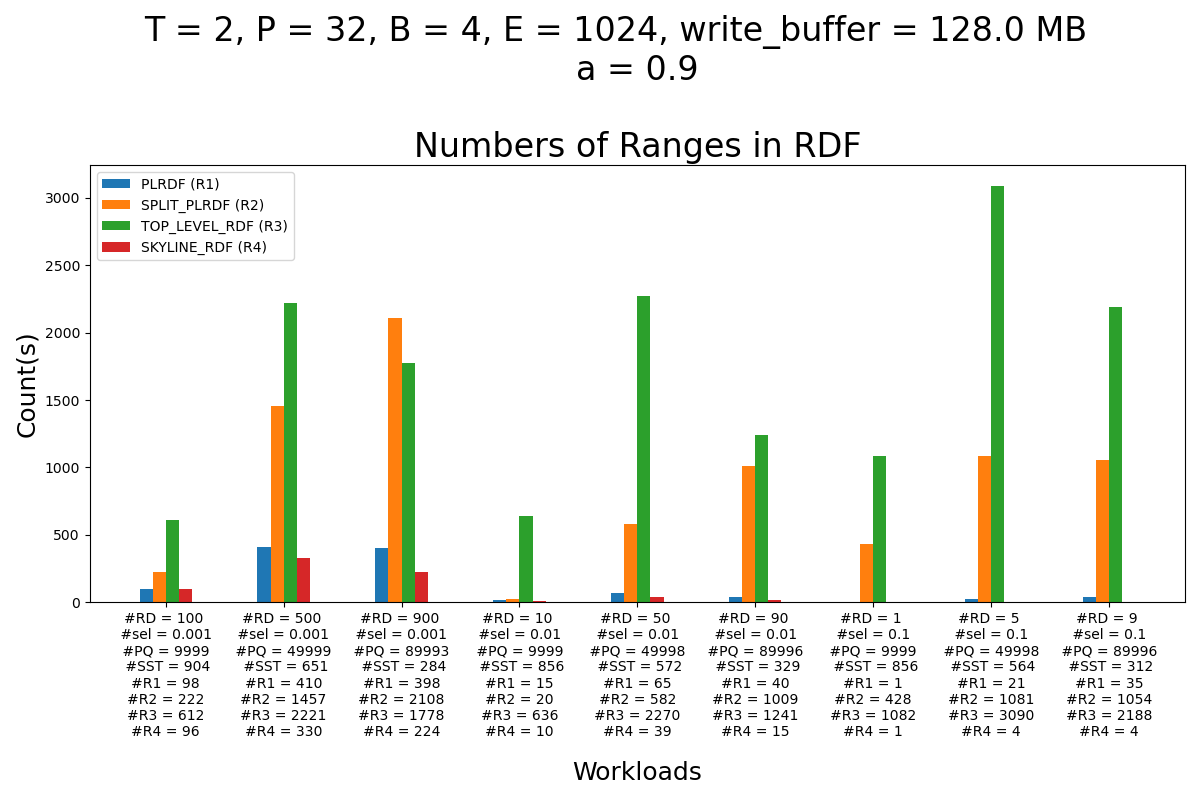
\includegraphics[scale=0.25]{Figures/T2_P32_B4_E1024_128p0MB_alpha0p9/T2_P32_B4_E1024_128p0MB_alpha0p9_Numbers_of_Ranges__Skyline.png}
    \Description[<short description>]{<long description>}
    \caption{ Number of ranges tested on all of the existing keys when $\alpha$ = 0.9, T = 2, P =32, E = 1024. Over 9 workloads.}
    \label{fig:numbers_of_Ranges__Skyline}
\end{figure}


\begin{figure}
    % \centering
    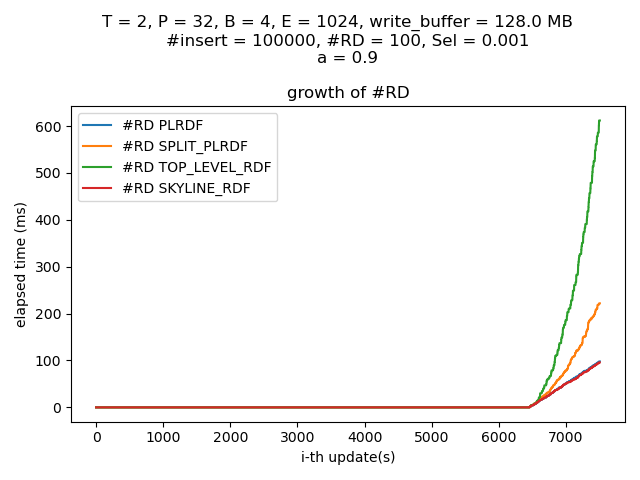
\includegraphics[scale=0.5]{Figures/T2_P32_B4_E1024_128p0MB_alpha0p9/T2_P32_B4_E1024_128p0MB_alpha0p9___I_100000_RD_100_Sel_0p001__alpha_0p9_growth_of_RDs.png}
    \Description[<short description>]{<long description>}
    \caption{ Numbers of ranges in RDs across time tested on all of the existing keys when $\alpha$ = 0.9, T = 2, P =32, E = 1024. Over 9 workloads.}
    \label{fig:growth_of_RDs__Skyline}
\end{figure}

In the following part, read buffer is disabled. And Point Query is performed after all the insertions has been done.

From Figure \ref{fig:elapsed_time__currently_deleted_keys__Skyline} and  Figure \ref{fig:elapsed_time__currently_deleted_keys}, one with SKyline and one without Skyline, we can see that the Skyline RDF is the worst of the all when performing PQ on the existing keys, because it doesn't return when the level contains RD, instead it only return when a key is found or going through all the levels. While the other RDF returns if they find a key is deleted by RD on a certain level. Comparing to Figure \ref{fig:elapsed_time__existing_keys__Skyline} which all the RDFs have similar work time, this is due to the fact that when performing PQ on existing keys, there's no chance of early return, which means that all doing the search until they reach the level where key lies. 

As the Figure \ref{fig:timing_breakdown__currently_deleted_keys__Skyline} shows, IOs occupies more than half of the time, if we can reduce the number of IOs, we can reduce the total query time.


Diving down to see the numbers of IOs spent on currently deleted keys in Figure \ref{fig:IO__currently_deleted_keys__Skyline} and Figure \ref{fig:IO__currently_deleted_keys}, there's no difference between PLRDF and default RocksDB implementation because when a file is opened the range deletes in a file are all read in to the buffer, when PQ is performed no extra IOs are spent to read in such meta data. Split\_PLRDF and TopLevel RDF have less IOs consumption as expected.


When the times goes by, the number of ranges in RDs increases with inserted keys, as Figure \ref{fig:growth_of_RDs__Skyline} shows, the number of ranges in RDs increases almost linearly. The ones split by the inserted points grows faster, and the TopLevel is the worst of all because it stays on the first level and never discard any ranges, while the ranges can be merged if there's a new range overlapped with the old ones.

At the end of the insert, numbers of ranges in RDs are shown in Figure 
\ref{fig:numbers_of_Ranges__Skyline}. Under most circumstances, TopLevel RDF is the worst for it keeps spliting and never discard any ranges. Skyline seems like the best while the PLRDF is almost comparable with the Skyline. When ranges are merged with a large input RD, numbers of ranges in TopLevel RDF may drops temporarily, but it will soon increase again.










\begin{figure}
    % \centering
    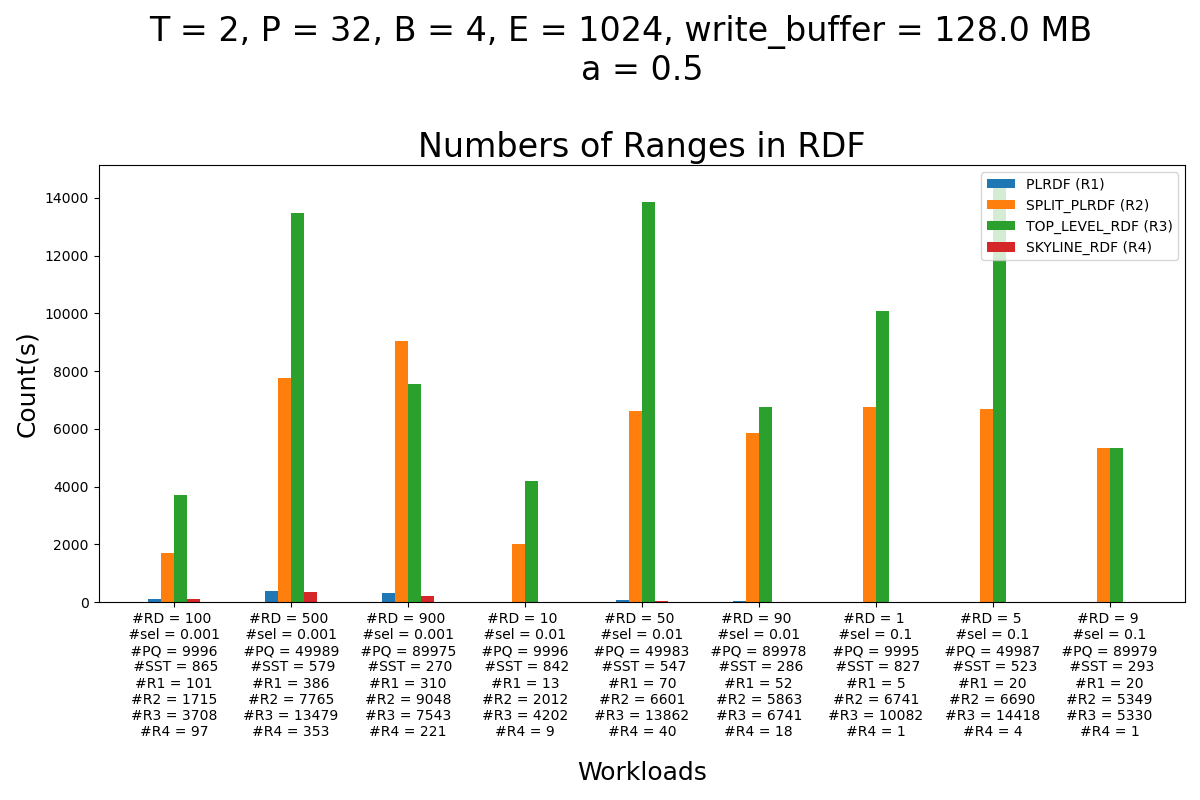
\includegraphics[scale=0.25]{Figures/T2_P32_B4_E1024_128p0MB_alpha0p5/T2_P32_B4_E1024_128p0MB_alpha0p5_Numbers_of_Ranges__Skyline.png}
    \Description[<short description>]{<long description>}
    \caption{\label{fig:numbers_of_Ranges_alpha_0.5__Skyline} Number of ranges tested on all of the existing keys when $\alpha$ = 0.5, T = 2, P =32, E = 1024. Over 9 workloads.}
\end{figure}


\begin{figure}
    % \centering
    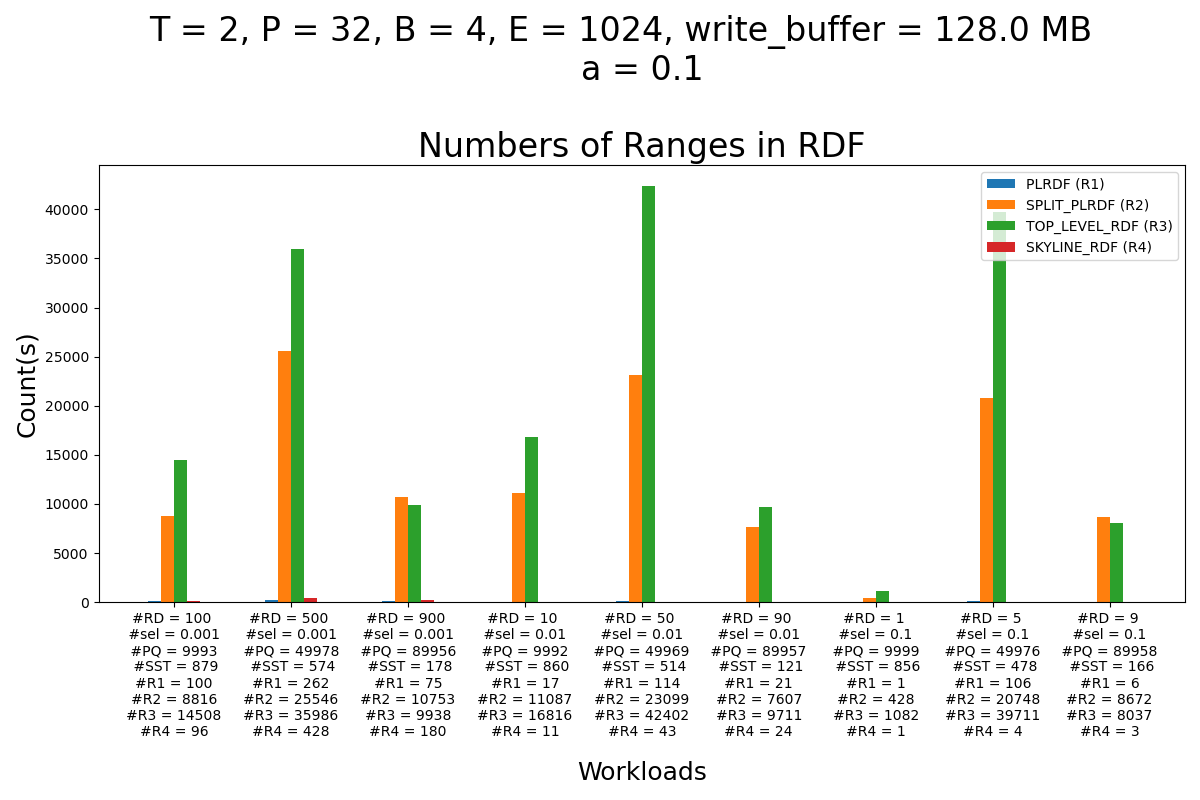
\includegraphics[scale=0.25]{Figures/T2_P32_B4_E1024_128p0MB_alpha0p1/T2_P32_B4_E1024_128p0MB_alpha0p1_Numbers_of_Ranges__Skyline.png}
    \Description[<short description>]{<long description>}
    \caption{\label{fig:numbers_of_Ranges_alpha_0.1__Skyline} Number of ranges tested on all of the existing keys when $\alpha$ = 0.1, T = 2, P =32, E = 1024. Over 9 workloads.}
\end{figure}



Now, when we decrease the value of alpha, making the first RD appeared earlier in the insertion workload, numbers of RDs increases, as in Figure \ref{fig:numbers_of_Ranges__Skyline}, \ref{fig:numbers_of_Ranges_alpha_0.5__Skyline} and Figure \ref{fig:numbers_of_Ranges_alpha_0.1__Skyline} with $\alpha$ being 0.9, 0.5, 0.1 respectively. The numbers can be 10 times larger.








% \begin{figure}
%     % \centering
%     
\includegraphics[scale=0.25]{Figures/T2_32P_B4_E1024_128p0MB_alpha0p9/T2_P32_B4_E1024_128p0MB_alpha0p9_elapse_time_on_currently_deleted_keys.png}
%     \Description[<short description>]{<long description>}
%     \caption{\label{fig:elapsed_time__currently_deleted_keys__B4_E1024} Number of ranges tested on all of the existing keys when $\alpha$ = 0.9, T = 2, P = 32, B = 4, E = 1024, write_buffer = 128 KB. Over 9 workloads.}
% \end{figure}

% \begin{figure}
%     % \centering
%     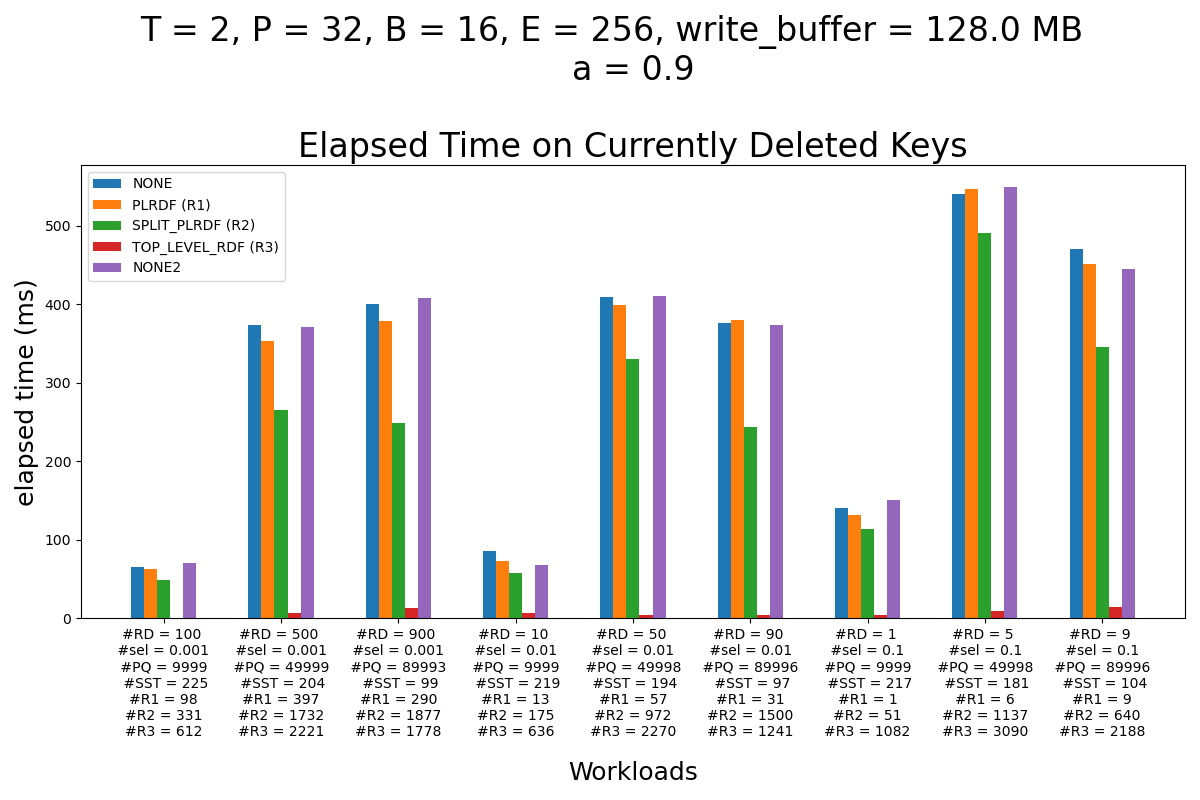
\includegraphics[scale=0.25]{Figures/T2_P32_B16_E256_128p0MB_alpha0p9/T2_P32_B16_E256_128p0MB_alpha0p9_elapse_time_on_currently_deleted_keys.png}
%     \Description[<short description>]{<long description>}
%     \caption{\label{fig:elapsed_time__currently_deleted_keys__B16_E256} Number of ranges tested on all of the existing keys when $\alpha$ = 0.9, T = 2, P = 32, B = 16, E = 256, write_buffer = 128 KB. Over 9 workloads.}
% \end{figure}

% \begin{figure}
%     % \centering
%     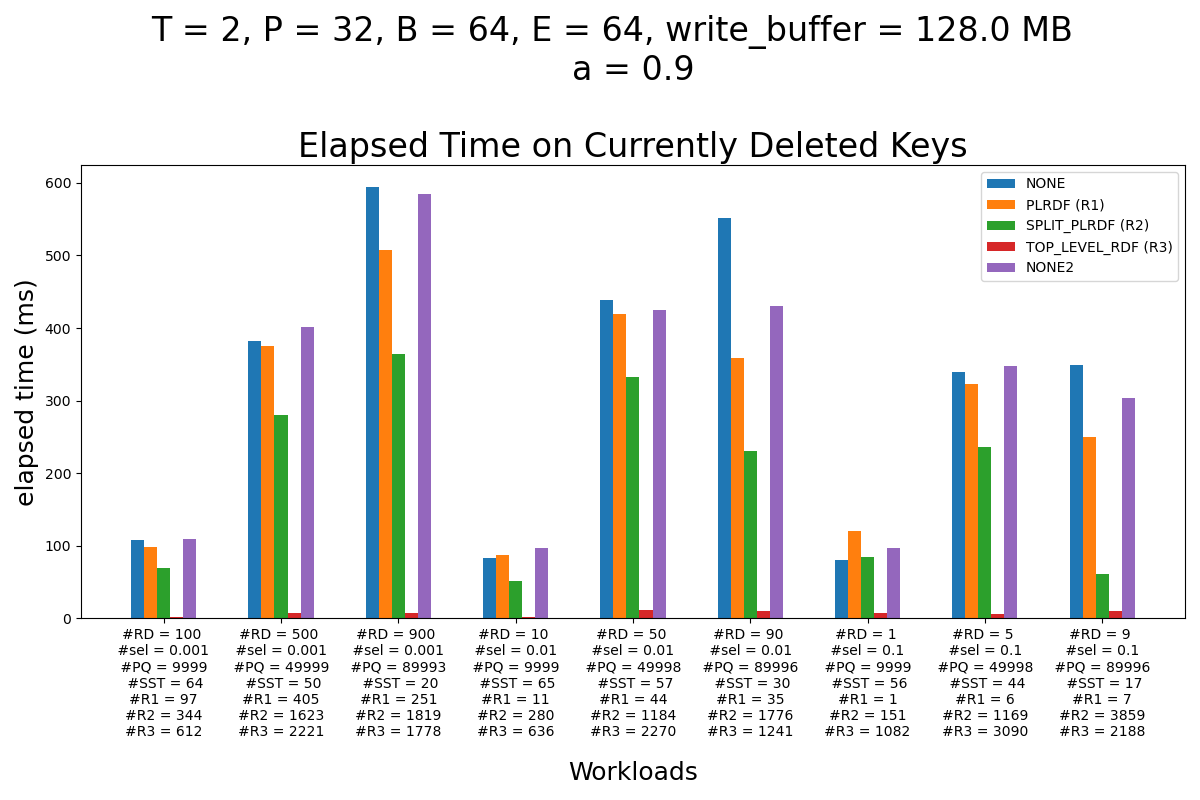
\includegraphics[scale=0.25]{Figures/T2_P32_B64_E64_128p0MB_alpha0p9/T2_P32_B64_E64_128p0MB_alpha0p9_elapse_time_on_currently_deleted_keys.png}
%     \Description[<short description>]{<long description>}
%     \caption{\label{fig:elapsed_time__currently_deleted_keys__B64_E64} Number of ranges tested on all of the existing keys when $\alpha$ = 0.9, T = 2, P = 32, B = 64, E = 64, write_buffer = 128 KB. Over 9 workloads.}
% \end{figure}









\begin{figure}
    % \centering
    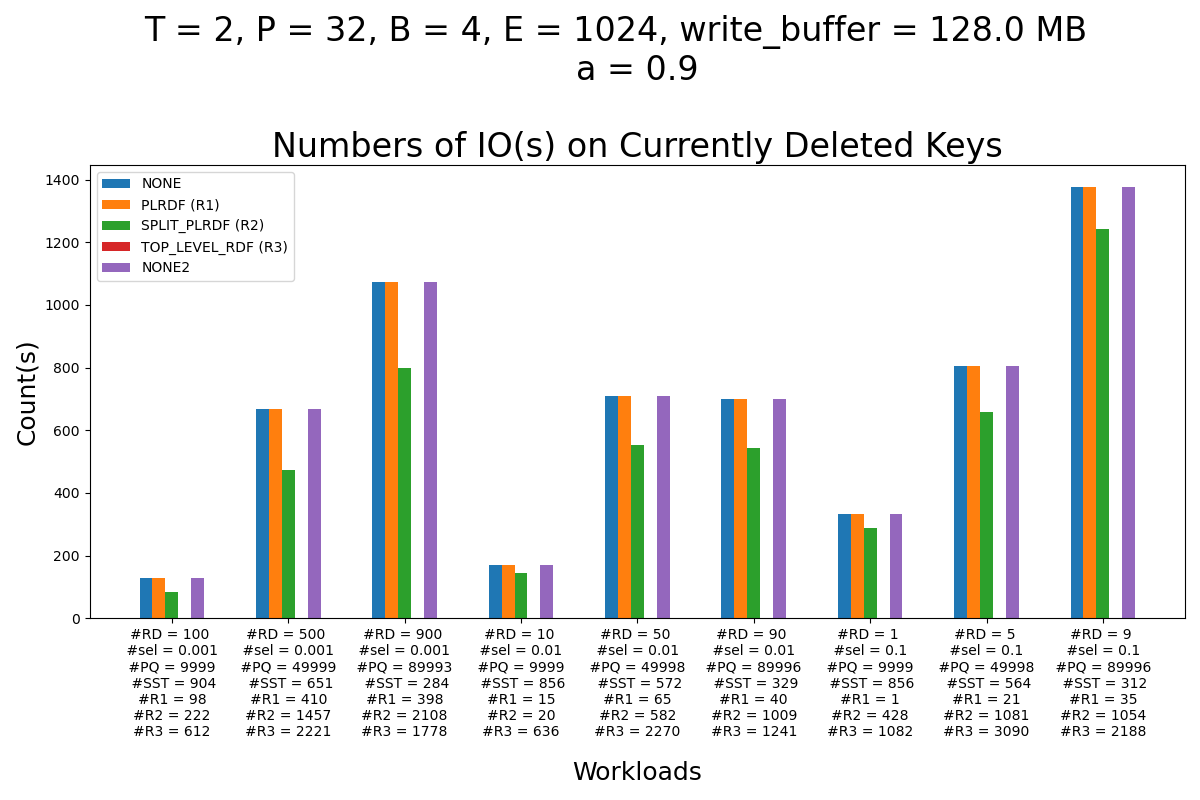
\includegraphics[scale=0.25]{Figures/T2_P32_B4_E1024_128p0MB_alpha0p9/T2_P32_B4_E1024_128p0MB_alpha0p9_IOs_on_currently_deleted_keys.png}
    \Description[<short description>]{<long description>}
    \caption{ Number of IOs tested on all of the existing keys when $\alpha$ = 0.9, T = 2, P = 32, B = 4, E = 1024. Over 9 workloads.}
    \label{fig:IOs__currently_deleted_keys__B4_E1024}
\end{figure}

\begin{figure}
    % \centering
    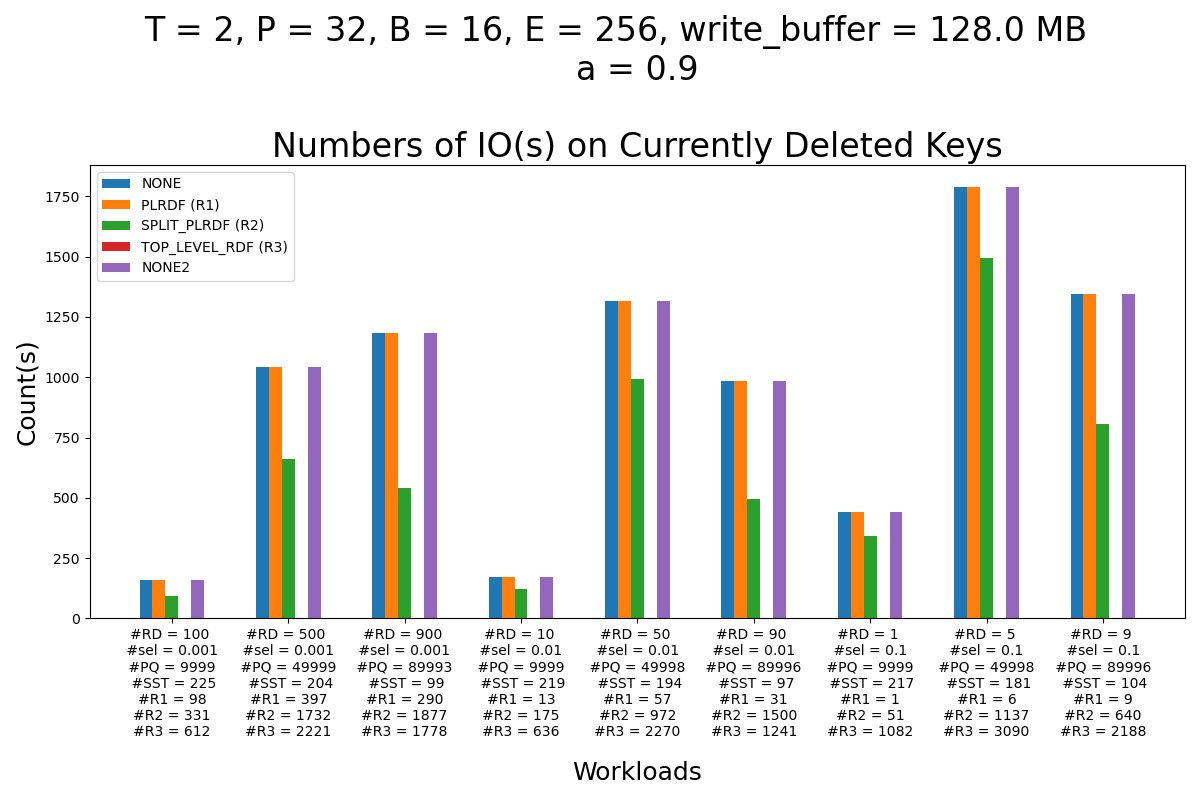
\includegraphics[scale=0.25]{Figures/T2_P32_B16_E256_128p0MB_alpha0p9/T2_P32_B16_E256_128p0MB_alpha0p9_IOs_on_currently_deleted_keys.png}
    \Description[<short description>]{<long description>}
    \caption{ Number of IOs tested on all of the existing keys when $\alpha$ = 0.9, T = 2, P = 32, B = 16, E = 256. Over 9 workloads.}
    \label{fig:IOs__currently_deleted_keys__B16_E256}
\end{figure}

\begin{figure}
    % \centering
    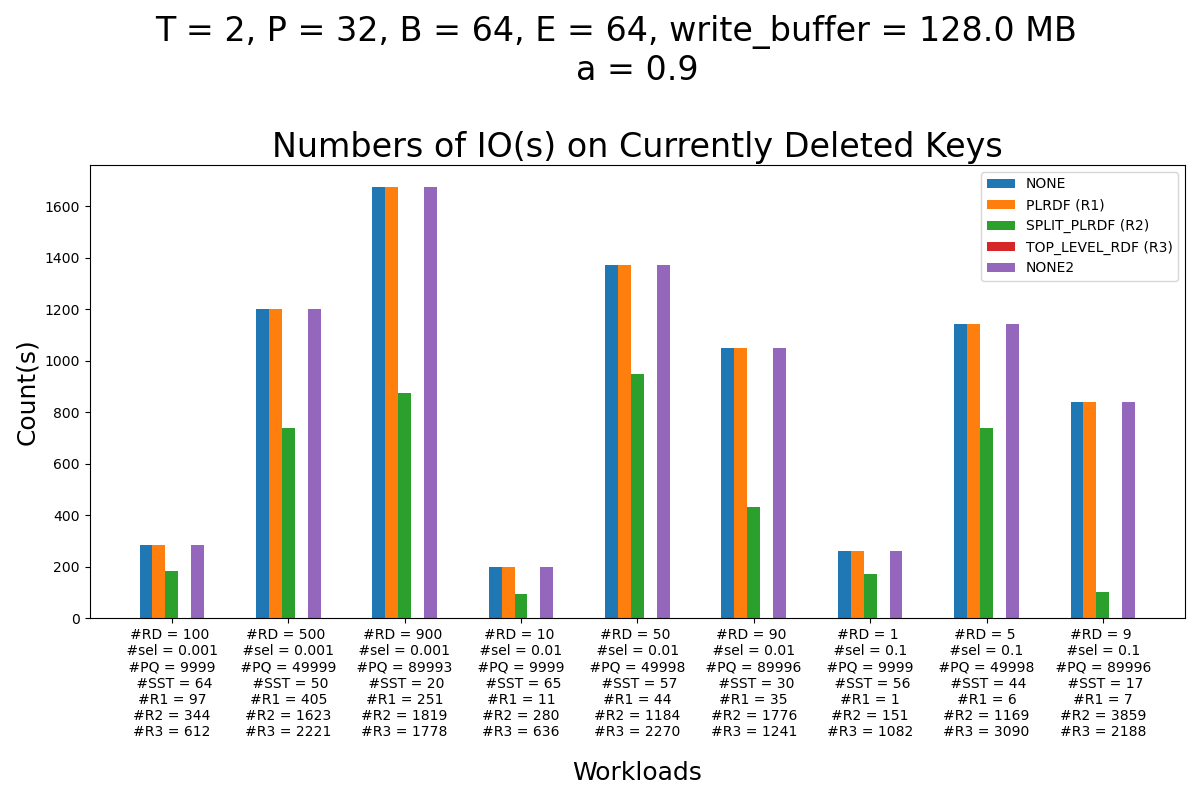
\includegraphics[scale=0.25]{Figures/T2_P32_B64_E64_128p0MB_alpha0p9/T2_P32_B64_E64_128p0MB_alpha0p9_IOs_on_currently_deleted_keys.png}
    \Description[<short description>]{<long description>}
    \caption{ Number of IOs tested on all of the existing keys when $\alpha$ = 0.9, T = 2, P = 32, B = 64, E = 64. Over 9 workloads.}
    \label{fig:IOs__currently_deleted_keys__B64_E64}
\end{figure}






% Comparing Figure \ref{fig:elapsed_time__currently_deleted_keys__B4_E1024}, \ref{fig:elapsed_time__currently_deleted_keys__B16_E256} and \ref{fig:elapsed_time__currently_deleted_keys__B64_E64}, we can see that when the sizes of pages and write buffers are fixed and varying on entry size, RDFs gain a small advantage when entry size becomes smaller, 


% Comparing Figure \ref{fig:IOs__currently_deleted_keys__B4_E1024}, \ref{fig:IOs__currently_deleted_keys__B16_E256} and \ref{fig:IOs__currently_deleted_keys__B64_E64}, we can see that when the sizes of pages and write buffers are fixed and only varying on entry size, RDFs gain a small advantage when entry size becomes smaller, total numbers of IOs decrease slightly.




\begin{figure*}[t!]
    \centering
    \begin{subfigure}{0.45\textwidth}
        \centering
        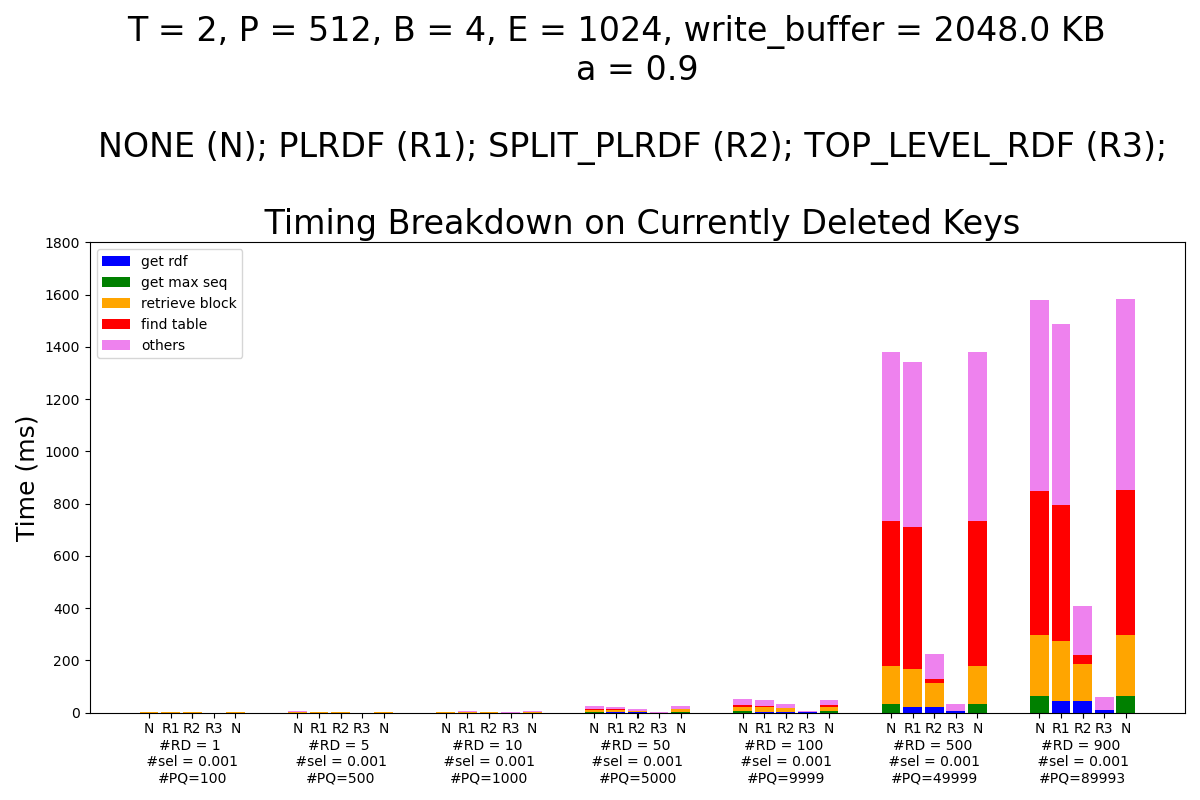
\includegraphics[height=1.8in]{Figures/Varying_on_numbers_of_RDs/T2_P512_B4_E1024_2048p0KB_alpha0p9/T2_P512_B4_E1024_2048p0KB_alpha0p9_timing_breakdown_on_currently_deleted_keys.png}
        \caption{ Timing breakdown, tested on all of the existing keys when $\alpha$ = 0.9, T = 2, P = 512, B = 4, E = 1024. Over 7 workloads.}
        \label{fig:elapsed_time__currently_deleted_keys__P512_B4_E1024__unnormalized}
    \end{subfigure}%
    ~ 
    % \vspace{1em}
    \hfill
    \begin{subfigure}{0.45\textwidth}
        \centering
        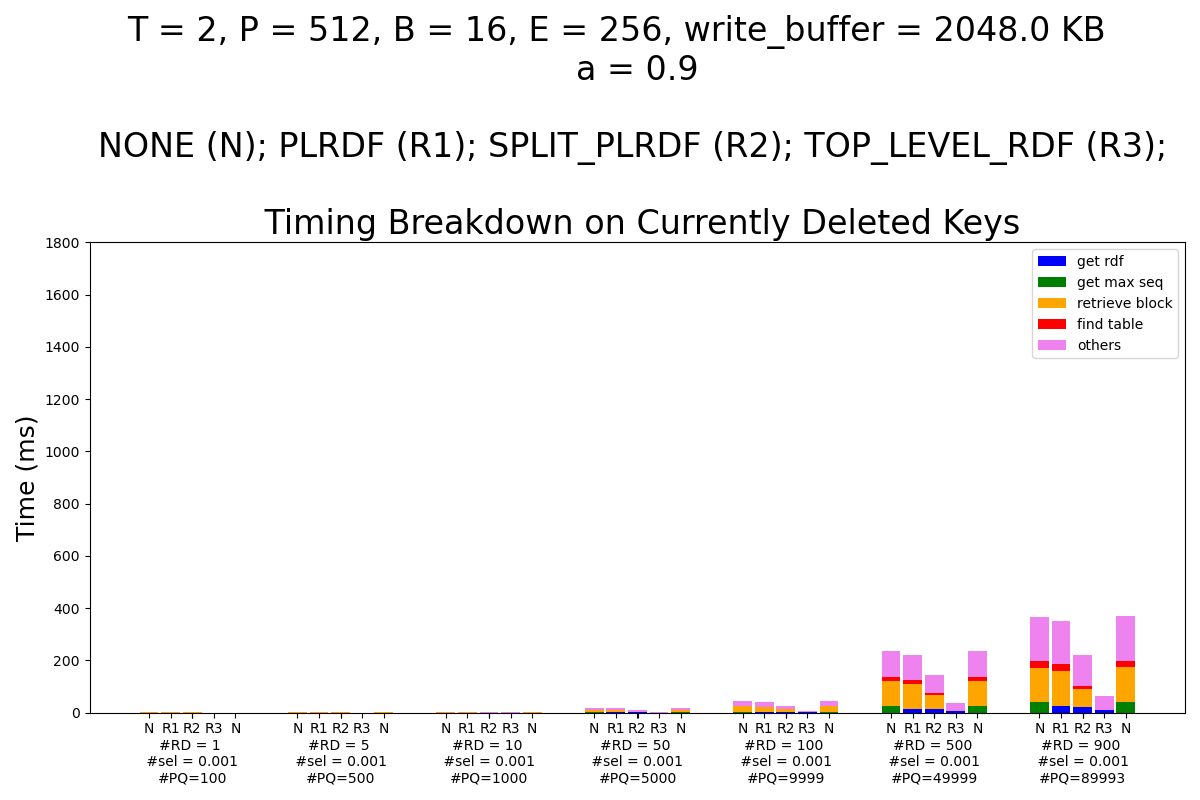
\includegraphics[height=1.8in]{Figures/Varying_on_numbers_of_RDs/T2_P512_B16_E256_2048p0KB_alpha0p9/T2_P512_B16_E256_2048p0KB_alpha0p9_timing_breakdown_on_currently_deleted_keys.png}
        \caption{ Timing breakdown, tested on all of the existing keys when $\alpha$ = 0.9, T = 2, P = 512, B = 16, E = 256. Over 7 workloads.}
        \label{fig:elapsed_time__currently_deleted_keys__P512_B16_E256__unnormalized}
    \end{subfigure}%
    % ~ 
    \vspace{1em}
    % \hfill
    \begin{subfigure}{0.45\textwidth}
        \centering
        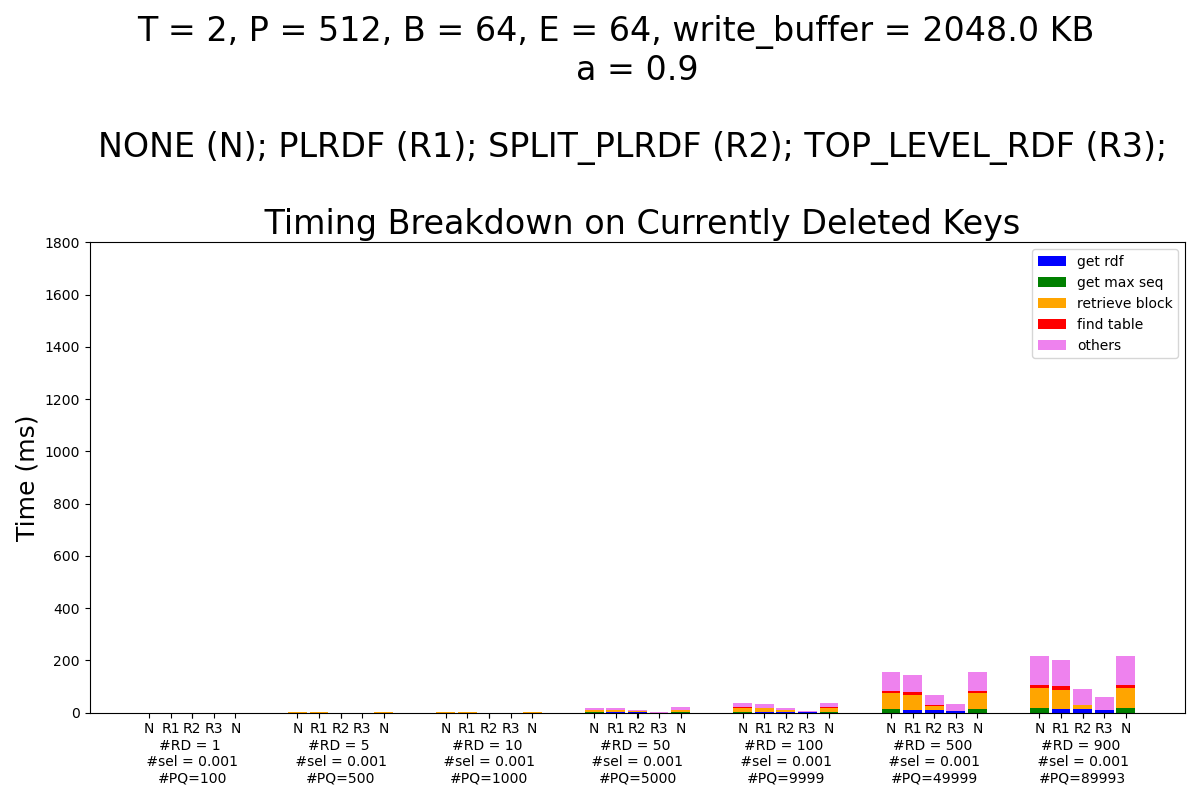
\includegraphics[height=1.8in]{Figures/Varying_on_numbers_of_RDs/T2_P512_B64_E64_2048p0KB_alpha0p9/T2_P512_B64_E64_2048p0KB_alpha0p9_timing_breakdown_on_currently_deleted_keys.png}
        \caption{ Timing breakdown, tested on all of the existing keys when $\alpha$ = 0.9, T = 2, P = 512, B = 64, E = 64. Over 7 workloads.}
        \label{fig:elapsed_time__currently_deleted_keys__P512_B64_E64__unnormalized}
    \end{subfigure}%
    ~ 
    % \vspace{1em}
    \hfill
    \begin{subfigure}{0.45\textwidth}
        \centering
        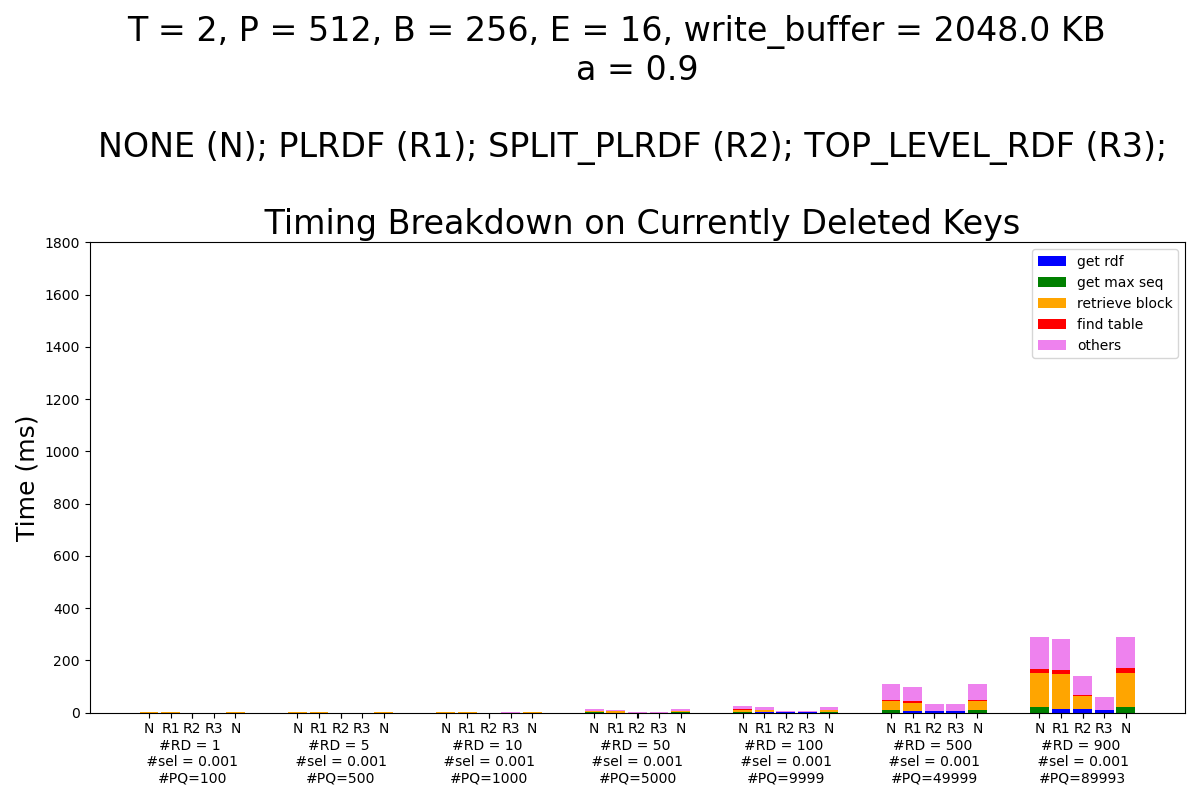
\includegraphics[height=1.8in]{Figures/Varying_on_numbers_of_RDs/T2_P512_B256_E16_2048p0KB_alpha0p9/T2_P512_B256_E16_2048p0KB_alpha0p9_timing_breakdown_on_currently_deleted_keys.png}
        \caption{ Timing breakdown, tested on all of the existing keys when $\alpha$ = 0.9, T = 2, P = 512, B = 256, E = 16. Over 7 workloads.}
        \label{fig:elapsed_time__currently_deleted_keys__P512_B256_E16__unnormalized}
    \end{subfigure}
    \caption{Unnormalized timing breakdown, varying on numbers of RDs for workload with $\alpha$ = 0.9, T = 2, P = 512, BxE = 4096.} 
    \label{fig:elapsed_time_breakdown__unnormalized__currently_deleted_keys__varying_on_numbers_of_RDs}
\end{figure*}



\begin{figure*}[t!]
    \centering
    \begin{subfigure}{0.45\textwidth}
        \centering
        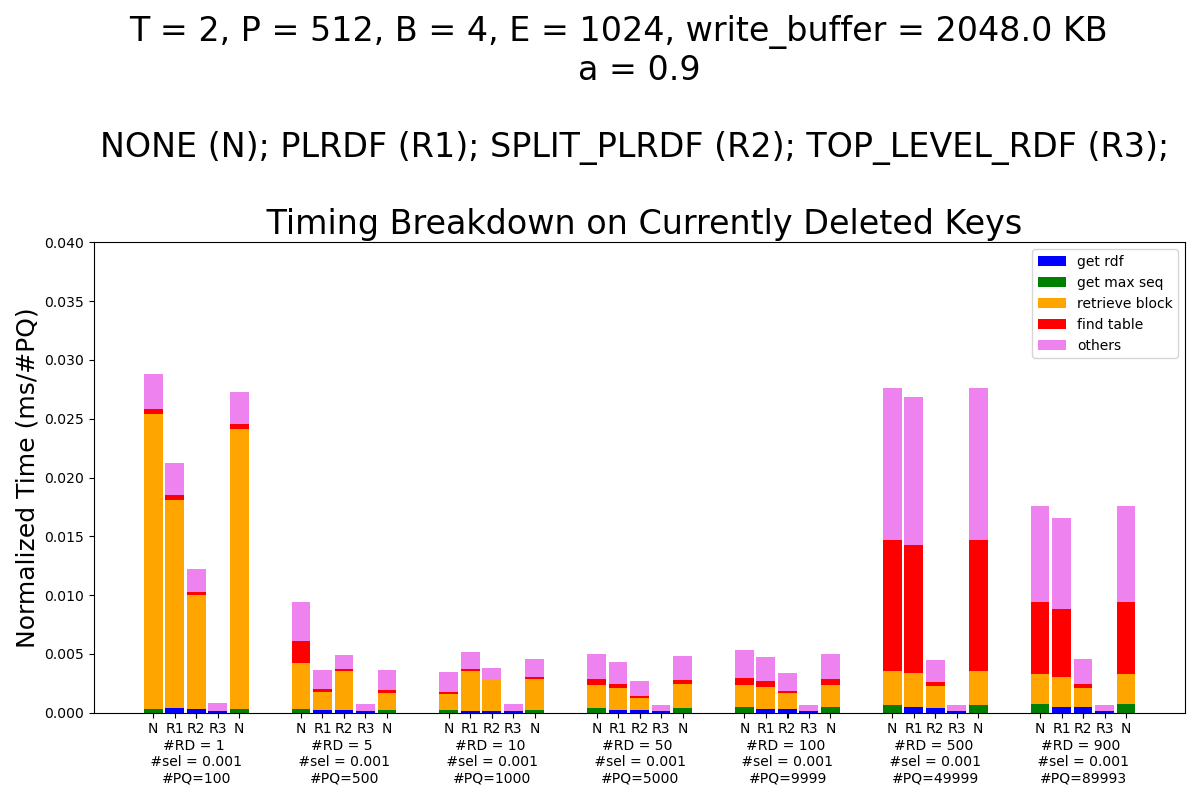
\includegraphics[height=1.8in]{Figures/Varying_on_numbers_of_RDs/T2_P512_B4_E1024_2048p0KB_alpha0p9/T2_P512_B4_E1024_2048p0KB_alpha0p9_timing_breakdown_on_currently_deleted_keys__normalized.png}
        \caption{ Timing breakdown, tested on all of the existing keys when $\alpha$ = 0.9, T = 2, P = 512, B = 4, E = 1024. Over 7 workloads.}
        \label{fig:elapsed_time__currently_deleted_keys__P512_B4_E1024__normalized}
    \end{subfigure}%
    ~ 
    % \vspace{1em}
    \hfill
    \begin{subfigure}{0.45\textwidth}
        \centering
        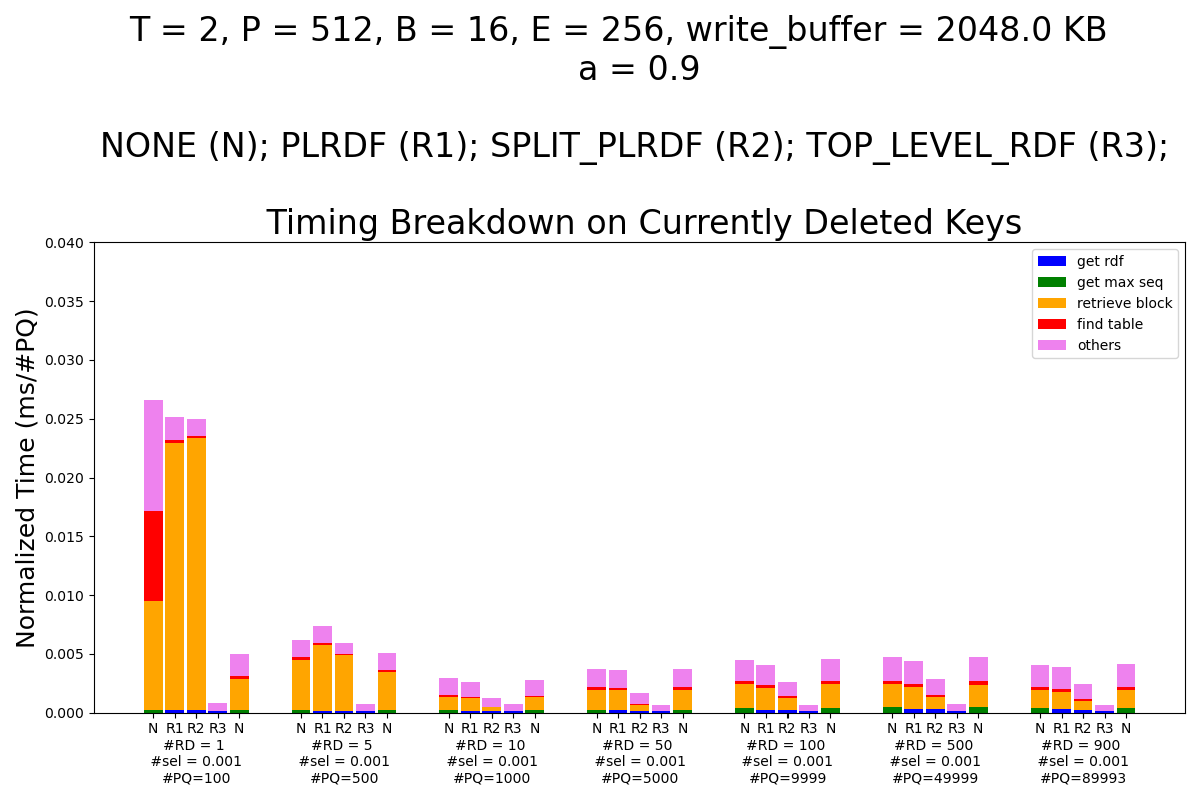
\includegraphics[height=1.8in]{Figures/Varying_on_numbers_of_RDs/T2_P512_B16_E256_2048p0KB_alpha0p9/T2_P512_B16_E256_2048p0KB_alpha0p9_timing_breakdown_on_currently_deleted_keys__normalized.png}
        \caption{ Timing breakdown, tested on all of the existing keys when $\alpha$ = 0.9, T = 2, P = 512, B = 16, E = 256. Over 7 workloads.}
        \label{fig:elapsed_time__currently_deleted_keys__P512_B16_E256__normalized}
    \end{subfigure}%
    % ~ 
    \vspace{1em}
    % \hfill
    \begin{subfigure}{0.45\textwidth}
        \centering
        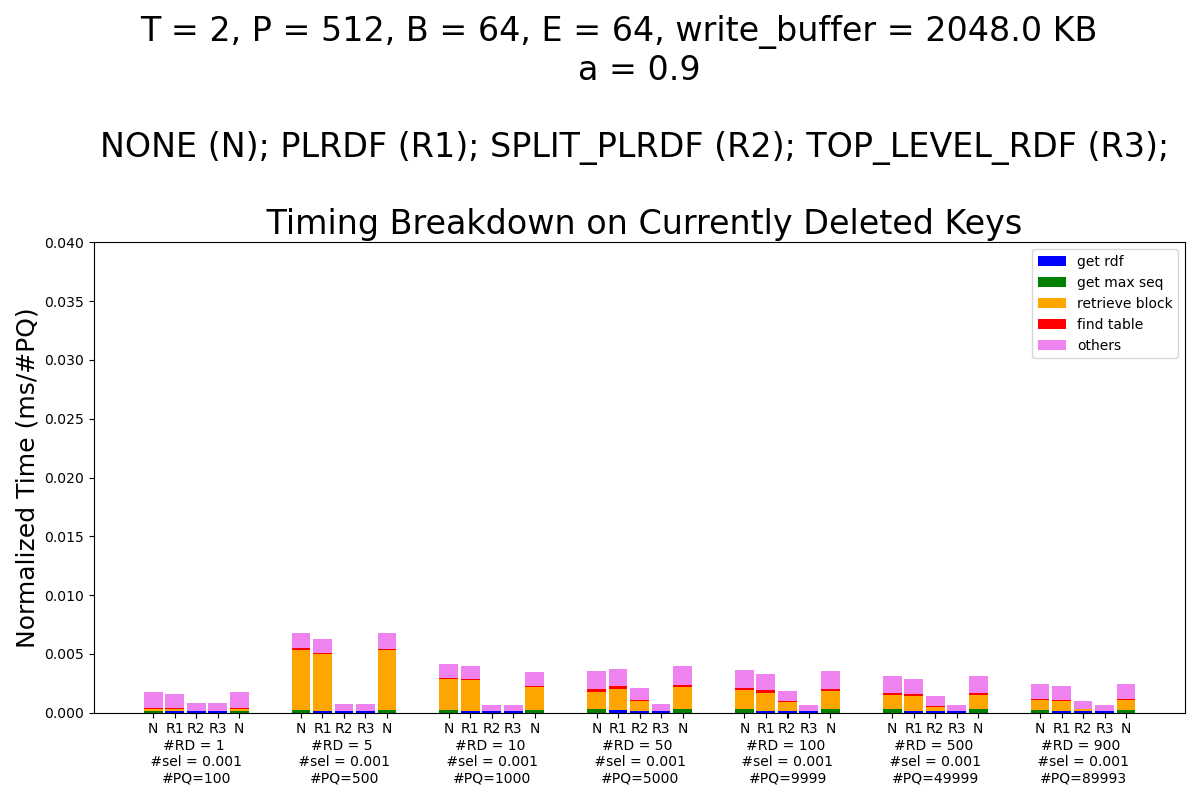
\includegraphics[height=1.8in]{Figures/Varying_on_numbers_of_RDs/T2_P512_B64_E64_2048p0KB_alpha0p9/T2_P512_B64_E64_2048p0KB_alpha0p9_timing_breakdown_on_currently_deleted_keys__normalized.png}
        \caption{ Timing breakdown, tested on all of the existing keys when $\alpha$ = 0.9, T = 2, P = 512, B = 64, E = 64. Over 7 workloads.}
        \label{fig:elapsed_time__currently_deleted_keys__P512_B64_E64__normalized}
    \end{subfigure}%
    ~ 
    % \vspace{1em}
    \hfill
    \begin{subfigure}{0.45\textwidth}
        \centering
        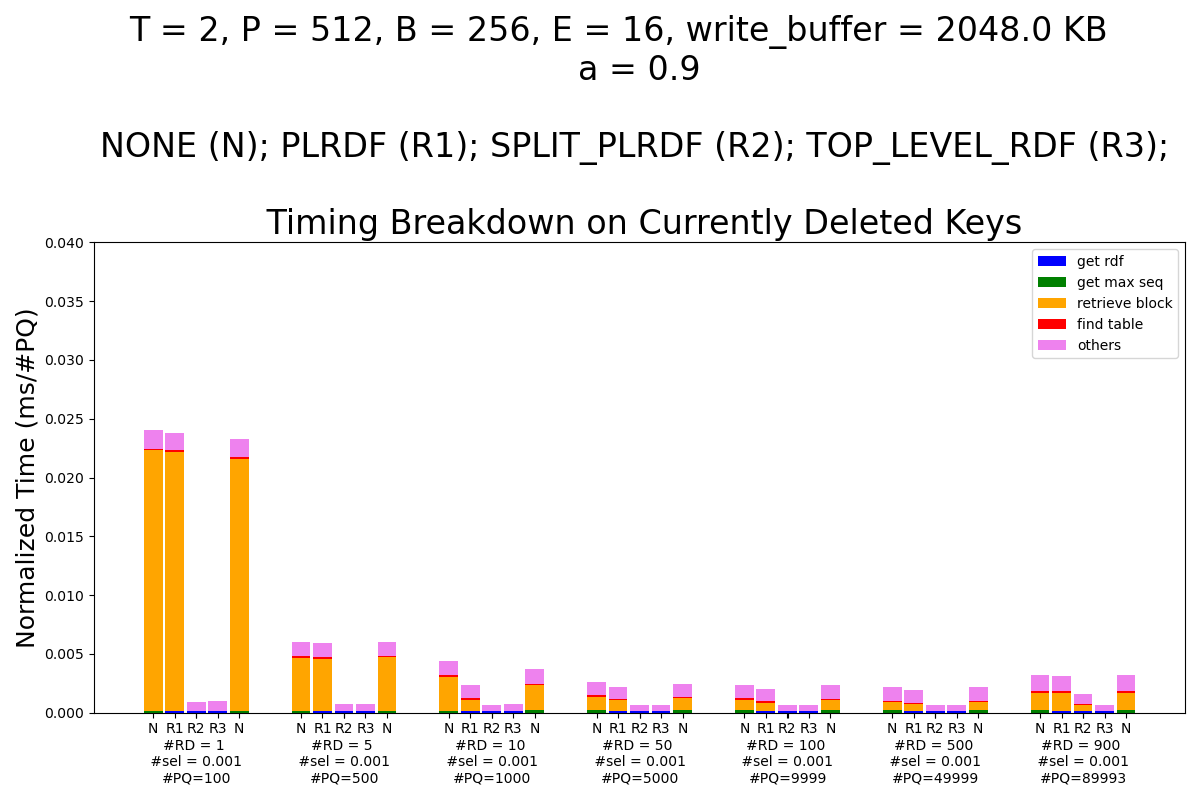
\includegraphics[height=1.8in]{Figures/Varying_on_numbers_of_RDs/T2_P512_B256_E16_2048p0KB_alpha0p9/T2_P512_B256_E16_2048p0KB_alpha0p9_timing_breakdown_on_currently_deleted_keys__normalized.png}
        \caption{ Timing breakdown, tested on all of the existing keys when $\alpha$ = 0.9, T = 2, P = 512, B = 256, E = 16. Over 7 workloads.}
        \label{fig:elapsed_time__currently_deleted_keys__P512_B256_E16__normalized}
    \end{subfigure}
    \caption{Normalized timing breakdown, varying on numbers of RDs for workload with $\alpha$ = 0.9, T = 2, P = 512, BxE = 4096.} 
    \label{fig:elapsed_time_breakdown__normalized__currently_deleted_keys__varying_on_numbers_of_RDs}
\end{figure*}



With Figure \ref{fig:elapsed_time_breakdown__unnormalized__currently_deleted_keys__varying_on_numbers_of_RDs} and Figure \ref{fig:elapsed_time_breakdown__normalized__currently_deleted_keys__varying_on_numbers_of_RDs}, we see when E becomes smaller, the total size of the file becomes smaller, so is the trend of the total elapsed time. While the percentage of CPU times comparing to Disk IOs time decreases too; This may cause by the fact that the retrieved data has to be processed.



	 
% \begin{figure*}[t!]
%     \centering
%     \begin{subfigure}{0.45\textwidth}
%         \centering
%         \includegraphics[height=1.8in]{Figures/Varying_on_selectivity/T2_P512_B4_E1024_2048p0KB_alpha0p9__varying_on_selectivity/T2_P512_B4_E1024_2048p0KB_alpha0p9__varying_on_selectivity_61x__timing_breakdown_on_currently_deleted_keys__normalized.png}
%         \caption{ Timing breakdown, tested on all of the existing keys when $\alpha$ = 0.9, T = 2, P = 512, B = 4, E = 1024. Over 7 workloads.}
%         \label{fig:elapsed_time__currently_deleted_keys__varying_on_selectivity_61x___P512_B4_E1024__normalized}
%     \end{subfigure}%
%     ~ 
%     % \vspace{1em}
%     \hfill
%     \begin{subfigure}{0.45\textwidth}
%         \centering
%         \includegraphics[height=1.8in]{Figures/Varying_on_selectivity/T2_P512_B16_E256_2048p0KB_alpha0p9__varying_on_selectivity/T2_P512_B16_E256_2048p0KB_alpha0p9__varying_on_selectivity_62x__timing_breakdown_on_currently_deleted_keys__normalized.png}
%         \caption{ Timing breakdown, tested on all of the existing keys when $\alpha$ = 0.9, T = 2, P = 512, B = 16, E = 256. Over 7 workloads.}
%         \label{fig:elapsed_time__currently_deleted_keys__varying_on_selectivity_62x___P512_B16_E256__normalized}
%     \end{subfigure}%
%     % ~ 
%     \vspace{1em}
%     % \hfill
%     \begin{subfigure}{0.45\textwidth}
%         \centering
%         \includegraphics[height=1.8in]{Figures/Varying_on_selectivity/T2_P512_B64_E64_2048p0KB_alpha0p9__varying_on_selectivity/T2_P512_B64_E64_2048p0KB_alpha0p9__varying_on_selectivity_63x__timing_breakdown_on_currently_deleted_keys__normalized.png}
%         \caption{ Timing breakdown, tested on all of the existing keys when $\alpha$ = 0.9, T = 2, P = 512, B = 64, E = 64. Over 7 workloads.}
%         \label{fig:elapsed_time__currently_deleted_keys__varying_on_selectivity_63x___P512_B64_E64__normalized}
%     \end{subfigure}%
%     ~ 
%     % \vspace{1em}
%     \hfill
%     \begin{subfigure}{0.45\textwidth}
%         \centering
%         \includegraphics[height=1.8in]{Figures/Varying_on_selectivity/T2_P512_B256_E16_2048p0KB_alpha0p9__varying_on_selectivity/T2_P512_B256_E16_2048p0KB_alpha0p9__varying_on_selectivity_64x__timing_breakdown_on_currently_deleted_keys__normalized.png}
%         \caption{ Timing breakdown, tested on all of the existing keys when $\alpha$ = 0.9, T = 2, P = 512, B = 256, E = 16. Over 7 workloads.}
%         \label{fig:elapsed_time__currently_deleted_keys__varying_on_selectivity_64x___P512_B256_E16__normalized}
%     \end{subfigure}
%     \caption{Normalized timing breakdown, varying on selectivity under numbers of RDs = 10 for workload with $\alpha$ = 0.9, T = 2, P = 512, BxE = 4096.} 
%     \label{fig:elapsed_time_breakdown__normalized__currently_deleted_keys__varying_on_selectivity}
% \end{figure*}


	 
% \begin{figure*}[t!]
%     \centering
%     \begin{subfigure}{0.45\textwidth}
%         \centering
%         \includegraphics[height=1.8in]{Figures/Varying_on_selectivity/T2_P512_B4_E1024_2048p0KB_alpha0p9__varying_on_selectivity/T2_P512_B4_E1024_2048p0KB_alpha0p9__varying_on_selectivity_51x__timing_breakdown_on_currently_deleted_keys__normalized.png}
%         \caption{ Timing breakdown, tested on all of the existing keys when $\alpha$ = 0.9, T = 2, P = 512, B = 4, E = 1024. Over 7 workloads.}
%         \label{fig:elapsed_time__currently_deleted_keys__varying_on_selectivity_51x___P512_B4_E1024__normalized}
%     \end{subfigure}%
%     ~ 
%     % \vspace{1em}
%     \hfill
%     \begin{subfigure}{0.45\textwidth}
%         \centering
%         \includegraphics[height=1.8in]{Figures/Varying_on_selectivity/T2_P512_B16_E256_2048p0KB_alpha0p9__varying_on_selectivity/T2_P512_B16_E256_2048p0KB_alpha0p9__varying_on_selectivity_52x__timing_breakdown_on_currently_deleted_keys__normalized.png}
%         \caption{ Timing breakdown, tested on all of the existing keys when $\alpha$ = 0.9, T = 2, P = 512, B = 16, E = 256. Over 7 workloads.}
%         \label{fig:elapsed_time__currently_deleted_keys__varying_on_selectivity_52x___P512_B16_E256__normalized}
%     \end{subfigure}%
%     % ~ 
%     \vspace{1em}
%     % \hfill
%     \begin{subfigure}{0.45\textwidth}
%         \centering
%         \includegraphics[height=1.8in]{Figures/Varying_on_selectivity/T2_P512_B64_E64_2048p0KB_alpha0p9__varying_on_selectivity/T2_P512_B64_E64_2048p0KB_alpha0p9__varying_on_selectivity_53x__timing_breakdown_on_currently_deleted_keys__normalized.png}
%         \caption{ Timing breakdown, tested on all of the existing keys when $\alpha$ = 0.9, T = 2, P = 512, B = 64, E = 64. Over 7 workloads.}
%         \label{fig:elapsed_time__currently_deleted_keys__varying_on_selectivity_53x___P512_B64_E64__normalized}
%     \end{subfigure}%
%     ~ 
%     % \vspace{1em}
%     \hfill
%     \begin{subfigure}{0.45\textwidth}
%         \centering
%         \includegraphics[height=1.8in]{Figures/Varying_on_selectivity/T2_P512_B256_E16_2048p0KB_alpha0p9__varying_on_selectivity/T2_P512_B256_E16_2048p0KB_alpha0p9__varying_on_selectivity_54x__timing_breakdown_on_currently_deleted_keys__normalized.png}
%         \caption{ Timing breakdown, tested on all of the existing keys when $\alpha$ = 0.9, T = 2, P = 512, B = 256, E = 16. Over 7 workloads.}
%         \label{fig:elapsed_time__currently_deleted_keys__varying_on_selectivity_54x___P512_B256_E16__normalized}
%     \end{subfigure}
%     \caption{Normalized timing breakdown, varying on selectivity under numbers of RDs = 100 for workload with $\alpha$ = 0.9, T = 2, P = 512, BxE = 4096.} 
%     \label{fig:elapsed_time_breakdown__normalized__currently_deleted_keys__varying_on_selectivity}
% \end{figure*}


